\chapter{REVISÃO BIBLIOGRÁFICA}
\label{rev_bib}
\section{\textbf{Introdução}}
Nesta seção é apresentada a literatura utilizada, analisando-se as partes pertinentes ao trabalho realizado. Os principais tópicos de estudo foram sobre os temas de \hyperref[sec_rev_MEF]{Método de Elementos Finitos}, \hyperref[sec_rev_MF]{Escoamentos Multifásicos}, \hyperref[sec_rev_EP]{Escoamentos Particulados em Turbomáquinas} e a \hyperref[sec_rev_POO]{Programação Orientada a Objeto}.

\section{\textbf{Método de Elementos Finitos}}
\label{sec_rev_MEF}
A representação matemática de fenômenos físicos é feita por equações, para certos casos esta representação pode ser realizada por uma equação linear simples, em outras situações ela é composta por equações diferenciais.

Infelizmente, nem todas equações possuem soluções analíticas, isto é, soluções contínuas em formas de equações.
Nestes casos, uma forma de encontrar algo que represente bem as observações reais realizadas é a solução numérica.
A solução numérica é uma aproximação do resultado real feito solucionando o problema em trechos discretos, de forma que quanto menor forem, maior será a precisão do resultado.

Os métodos utilizados neste trabalho são conhecidos como: o Método das Diferenças Finitas (\textbf{MDF}) e o Método dos Elementos Finitos (\textbf{MEF}).

O Método de Diferenças Finitas foi um dos primeiros métodos numéricos a serem desenvolvidos, apresentado por Courant et. al. (1928)\cite{Courant-1928}, sua metodologia é realizada a partir da discretização da equação de governo do problema em diferenças discretas, dividindo-se o domínio contínuo em regiões pontuais.
De forma que quanto menor for o espaçamento entre as regiões do domínio mais preciso o método se tornará.
A razão matemática deste mecanismo pode ser interpretada com a definição da derivada, que busca representar a taxa de variação contínua em um ponto tomando-se o limite da diferença entre o valor da função em dois pontos sobre a distância entre os mesmos, quando esta distância se aproxima a zero.
As fórmulas de discretização das equações são baseadas na expansão da Série de Taylor como aplicado por George Boole (1859)\cite{Boole-1859}.
O operador diferencial é substituído por uma soma aproximadamente equivalente, com a ordem de seu erro sendo relativo ao número de termos.
Dentro desta substituição podem ser escolhidos vários esquemas, cada um com suas aplicações, vantagens e desvantagens.
Os esquemas mais usuais são os de diferenças atrasadas (\textit{Backwards Differences}), diferenças adiantadas (\textit{Forward Differences}) e diferenças centradas (\textit{Central Differences}), onde, em geral, as diferenças centradas possuem melhor aproximação.

Em seguida, os estudos sobre o Método de Elementos Finitos foram iniciados posteriormente e no início de seu desenvolvimento foi voltado para a solução de sistemas mais complexos, que incluíam equações diferenciais parciais.
Seus primeiros trabalhos na área da engenharia estudavam as soluções de problemas em sólidos e estruturas em geral como estudado por Turner (1956)\cite{Turner-1956}.
Sua metodologia funciona de forma similar porém, é um processo mais complexo pois trata-se em dividir o domínio em regiões pontuais interligadas, chamadas de nós.
As equações do sistema são aplicadas a cada nó e sua influência é transmitida para seus nós vizinhos.
Um grupo de nós gera o que é chamado de elemento, estes elementos podem estar organizados com diversas formas geométricas: triângulos, quadriláteros, pentágonos, etc.
O espaçamento entre os nós pode ser constante ou não, estruturada e não-estruturada, respectivamente.
O domínio onde estes elementos são definidos e estão contidos é chamado de malha.

A metodologia deste método, de acordo com Lewis et. al. (2004)\cite{lewis}, consiste na reformulação da equação de governo no que é chamada de forma fraca.
Esta forma é obtida realizando-se primeiro a conversão do problema para a forma forte, que se trata da avaliação das equações com funções peso atribuídas.
Estas funções peso são arbitrárias e são escolhidas de acordo com o método de discretização utilizado.
Durante a conversão das equações para a forma forte, surgem as chamadas funções base, de forma ou interpoladoras, estas servem como determinadores das componentes do valor da função em cada nó dentro do elemento.
Existem diversos esquemas para a escolha das funções de peso, os mais comuns na literatura são os esquemas de: Galerkin, Taylor-Galerkin e Petrov-Galerkin.
Neste trabalho será utilizado o método de Galerkin, que define as funções de peso com mesmo valor das funções de base.
Em seguida, a formulação forte é integrada sobre o domínio para se encontrar a forma fraca do problema.

Após encontrar a forma fraca, ela é transformada em sua versão matricial para cada elemento, onde cada índice corresponde a um nó local presente no elemento.
Em seguida estas matrizes são adicionadas a uma matriz global que representa a componente de cada nó presente no domínio.
Então são aplicadas as condições de contorno e o sistema é resolvido, obtendo-se o valor da variável da equação governante em cada nó da malha.

Assim como estudado por Carnevale (2018)\cite{carnevale}, será utilizada a formulação de corrente-vorticidade como uma alternativa a equação de Navier-Stokes.
Embora neste trabalho, há um foco maior em escoamentos multifásicos com partículas e na aplição do código como uma biblioteca livre, e portanto seu código é desenvolvido de outra maneira.

Dentro da seleção do comportamento da malha pode-se escolher entre esquemas que consideram a malha fixa, chamada de formulação Euleriana, esquemas com a malha móvel, chamada de formulação Lagrangiana, e esquemas mistos como o chamado Lagrangiano-Euleriano Arbitrário (ALE) como explicado por Anjos et. al. (2015)\cite{ALE-2015}.
Neste trabalho será utilizado o esquema de Euler, onde a malha é considerada estacionária e o valor das variáveis de campo de interesse são calculados na posição dos nós da malha.
Para a geração dos pontos e elementos da malha será utilizado o \textit{software open source \href{http://gmsh.info}{Gmsh}}, como sugerido por Geuzaine e Remacle (2009)\cite{gmsh}.

\section{\textbf{Escoamentos Multifásicos}}
\label{sec_rev_MF}
Escoamentos multifásicos são utilizados largamente na área da engenharia para uma diversidade de aplicações.
Estes ocorrem quando há o transporte de mais de uma substância em fases não miscigenadas.
Estas fases podem estar ou não no mesmo estado, subdividindo os tipos de escoamento multifásico no tipo de interação entre as fases, líquido-líquido, gás-líquido e sólido-líquido.

Dentro da engenharia mecânica pode-se verificar a grande importância destes escoamentos em casos como a extração de petróleo, onde é injetado um fluido e é captada uma mistura deste com o óleo bruto, e em trocadores de calor que possuem interação entre os fluidos.

Para os escoamentos particulados, sólido-líquido ou sólido-gás com pequenos sólidos chamados de partículas, pode-se notar sua importância até mesmo no transporte de dejetos, na área de saneamento.%, com os chamados escoamentos de superfície livre.
Alguns exemplos na seção de mecânica incluem o transporte de vapor com condensado, formação de bolhas em bombas e sólidos precipitados.

Um dos primeiros trabalhos sobre este tipo de escoamento foi Baker et al. (1965)\cite{Baker-1965}, sobre o comportamento de escoamentos multifásicos em transportes verticais.
Estes usados bastante em trocadores de calor, para melhorar sua eficiência de troca térmica.

%Um dos tipos de escoamentos multifásicos é o escoamento particulado, sólido-líquido ou sólido-gás, que é o foco deste trabalho.
Elghobashi et al. (1991)\cite{Elghobashi-1991} estuda o comportamento de escoamentos particulados demonstrando o efeito da turbulência na simulação de escoamentos multifásicos.

Como apresentado por Balachandar et al. (2010)\cite{Balachandar-2010}, os valores da fração de volume ocupada pela fase dispersa e a razão entre a massa da fase dispersa e a massa da fase líquida servem como indicadores do nível de interação entre as fases.
Para valores muito pequenos, o efeito dominante é do escoamento, portanto, neste caso pode-se considerar apenas os efeitos do fluido sobre as partículas, chamado de \textit{one-way flow}.
Para casos com valores maiores, as partículas tomam um papel mais significativo no escoamento e é preciso fazer uma ligação recíproca entre os mesmos.
Portanto, recalcula-se o escoamento considerando os efeitos das partículas no fluido, conhecido como de \textit{two-way flow}.
Finalmente, quando estes valores forem mais elevados a fase particulada toma um papel importante no comportamento e torna-se necessário considerar até os efeitos de outras partículas sobre cada uma delas, como colisão, aglomeração e quebra, denominado por Elghobashi et al. (1994)\cite{Elghobashi-1994} de \textit{four-way flow}.

Para a modelagem das forças atuando sobre cada partícula no escoamento foi utilizada a equação \textbf{Basset–Boussinesq–Oseen} (BBO), apresentada por Shao-Lee Soo et al. (1999)\cite{ShaoLeeSoo-1999}.
Esta equação é subdivida em várias forças atuantes, como a gravidade, arrasto, massa virtual, entre outras.
Entretanto, as equações das forças possuem uma restrição para sua validade, podendo apenas serem aplicadas para casos com baixo número de Reynolds.


\section{\textbf{Escoamentos Particulados em Turbomáquinas}}
\label{sec_rev_EP}
Dentro do ciclo de vida de uma turbomáquina, pode-se esperar um certo desgaste devido a pequenas partículas que se chocam contra as paredes durante o movimento do rotor.
Este desgaste está ligado as propriedades do escoamento assim como das partículas.

Este efeito está presente até em turbinas de aeronaves, como estudado por Hussein et al. (1973)\cite{Hussein-1973}.
Este tipo de escoamento sólido-gás é verificado em locais com altos níveis de poluição.
Pode-se encontrar pequenas partículas sólidas presentes no ar ingerido por turbinas industriais e de aeronaves.
A sua presença causa um desgaste acelerado nas regiões radiais da turbina, como verificado também por Tabakoff et al. (1986)\cite{Tabakoff-1986}, que apresentou as zonas de maior colisão das partículas.
Estes trabalhos lidam diretamente com os efeitos da colisão das partículas, utilizando modelos que representam o comportamento delas após o choque.

Entrando na área de sólido-líquido, Uzol et al. (2002)\cite{Uzol-2002} fez um estudo mostrando o escoamento de uma turbomáquina utilizando partículas inseridas e um velocímetro de imagem para acompanhar seu trajeto.
Este trabalho não estuda o especificamente um escoamento particulado experimental, porém, utiliza alguns exemplos como ferramenta para visualizar seu comportamento para casos em geral.

Em Ghenaiet et al. (2005)\cite{Ghenaiet-2005} é estudado com mais profundidade os efeitos dos escoamentos particulados em turbomáquinas com líquidos.
Neste caso, é estudado os efeitos da degradação causada por partículas de areia ingeridas pelo escoamento no desempenho de uma turbomáquina axial.
Foi criado um modelo preditivo e demonstrada uma correlação entre o tamanho das partículas e a velocidade da degradação causada.

A causa mais comum de erosão em impelidores de turbomáquinas trabalhando com líquidos é a cavitação.
A cavitação é a formação de bolhas de ar devido a uma queda local na pressão que logo após serem geradas implodem, gerando ondas de vibração e podendo danificar locais próximos.
A \ref{JAC-Pump} mostra os efeitos do desgaste causado pelo efeito da cavitação em uma bomba.
\begin{figure}[H]
    \centering
    \stackunder{
        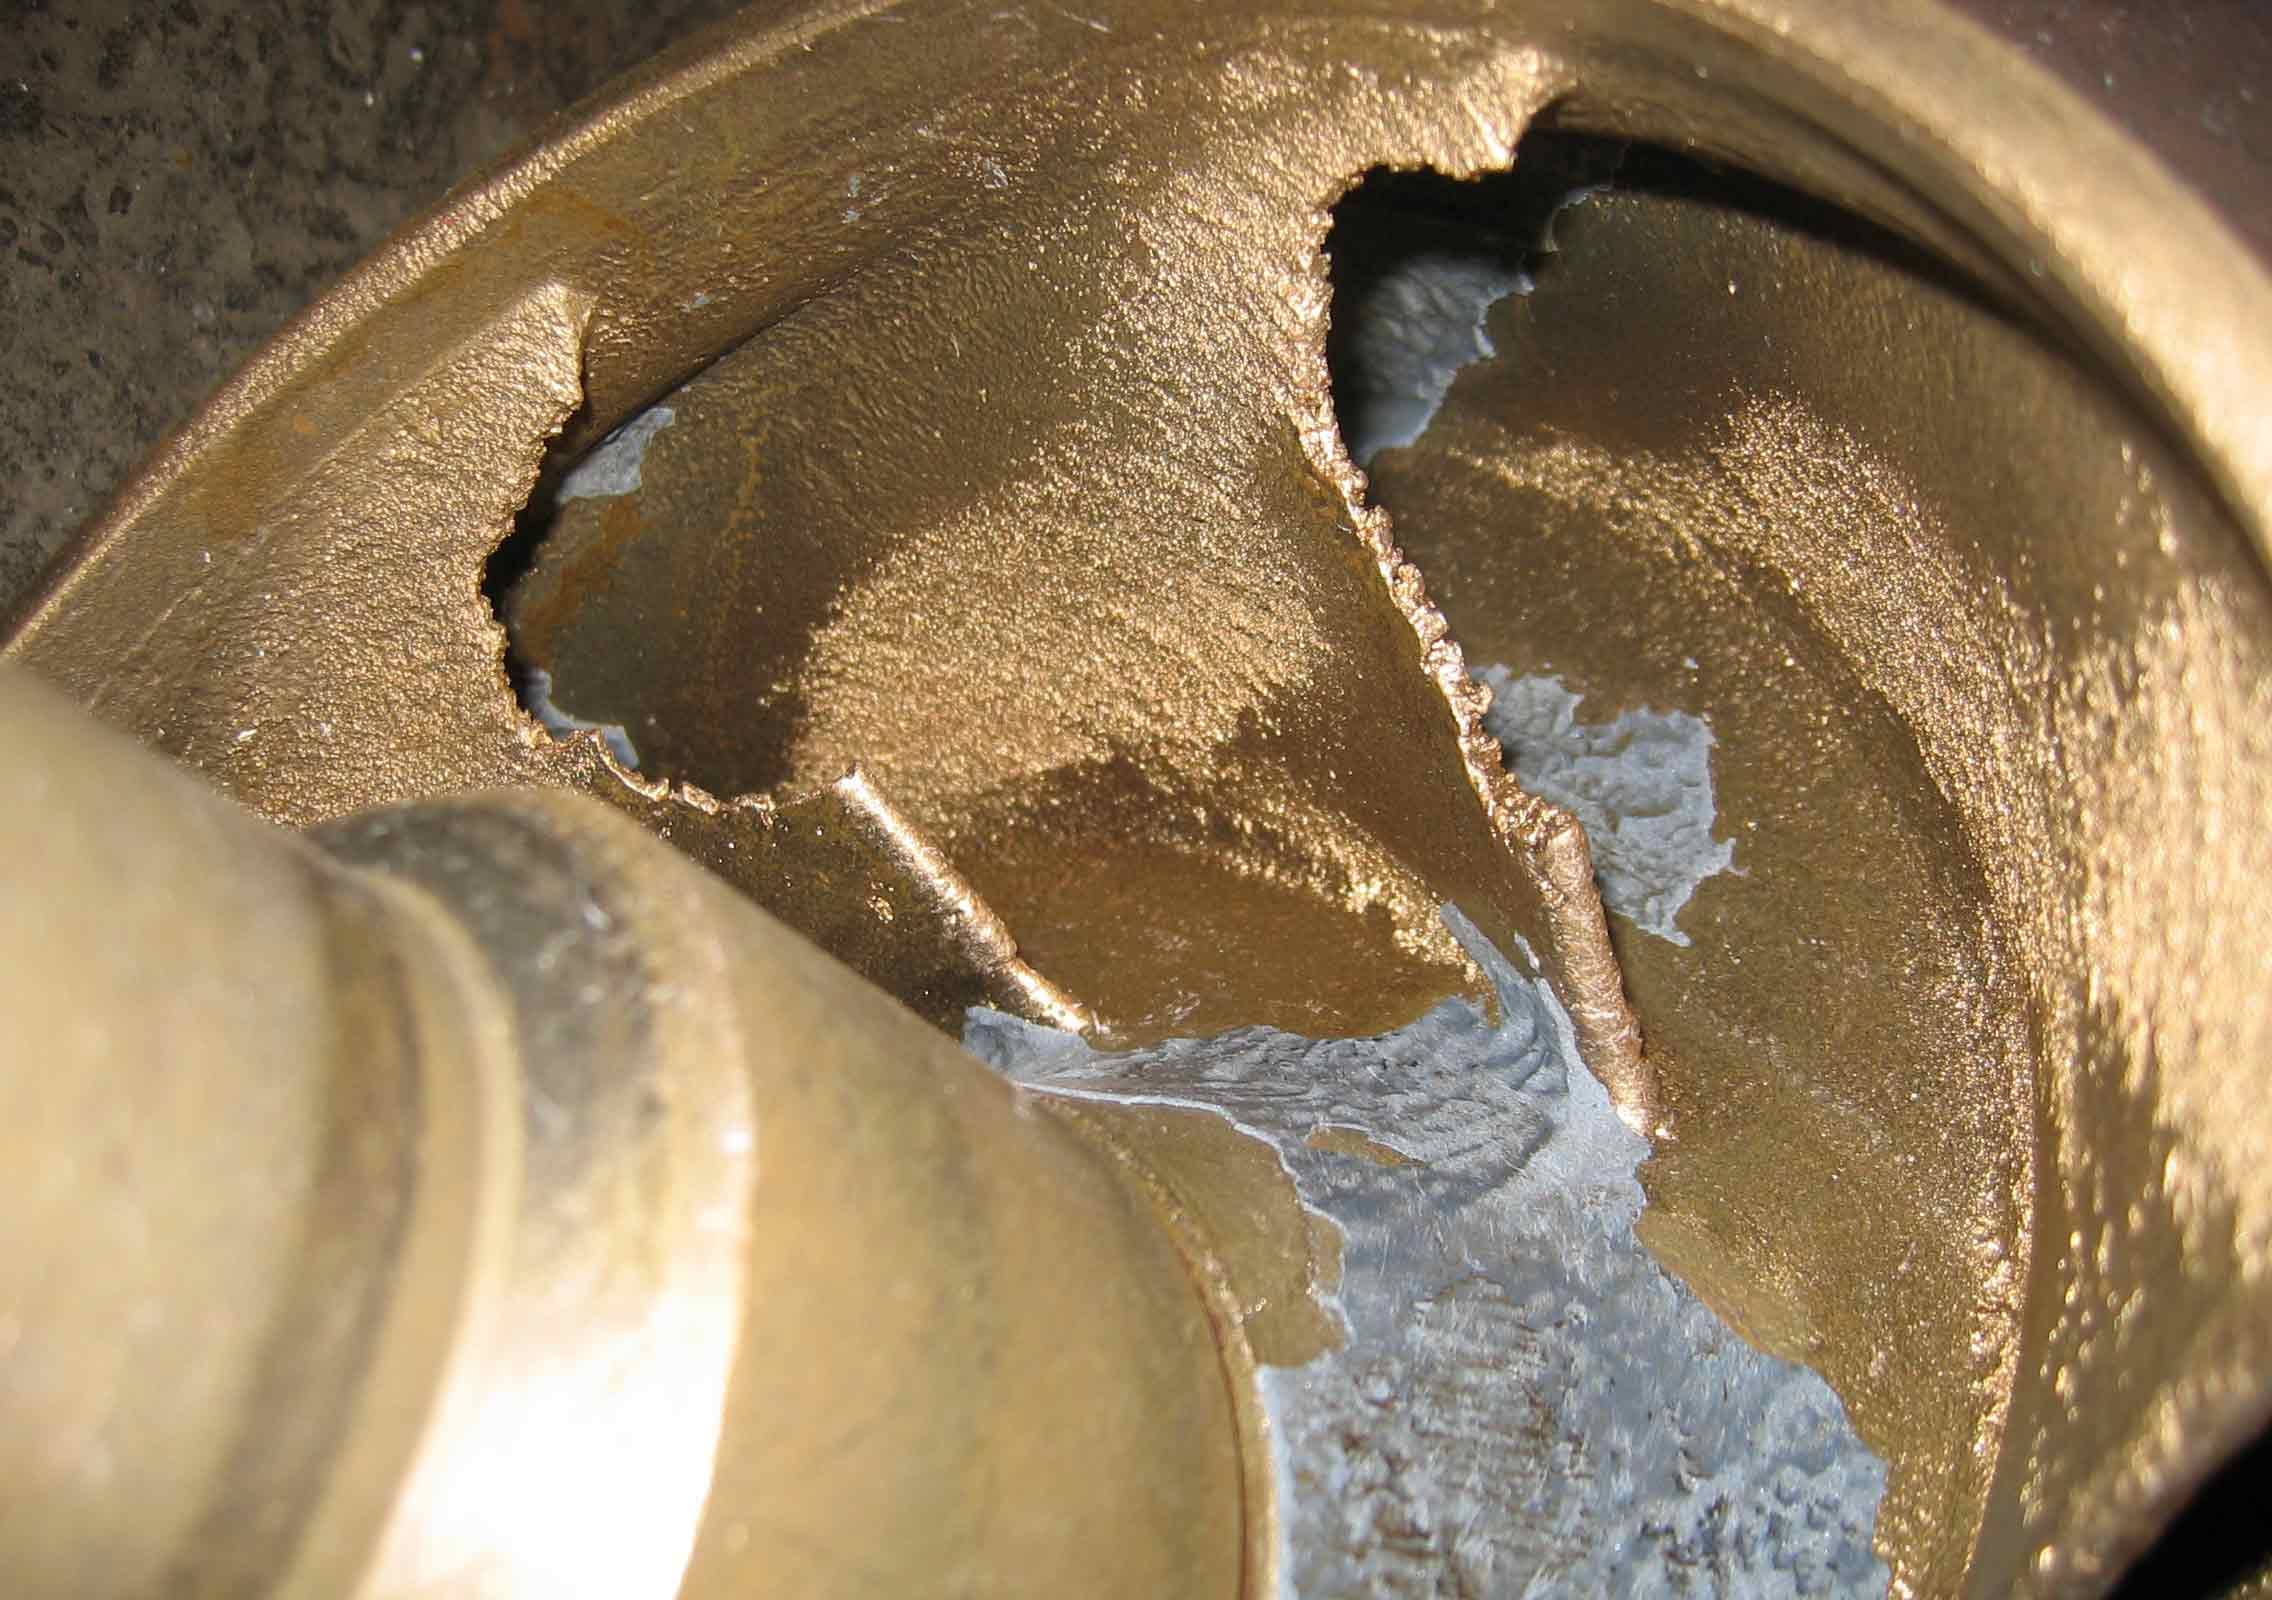
\includegraphics[width=0.6\linewidth]{figures/thermalchgo-017w2.jpg}
    } {\raggedleft \scriptsize Fonte: John Anspach Consulting\cite{JAC}.}
    \caption{Erosão em um impelidor causada pela cavitação.}
    \label{JAC-Pump}
\end{figure}

Blake et al. (1987)\cite{Blake-1987} estudou o comportamento da cavitação tomando o ponto de vista das bolhas criadas como partículas no escoamento.
Através desta interpretação, pode-se realizar simulações dos efeitos da cavitação com modelos de escoamentos particulados.
Porém neste trabalho não será realizada esta análise, visando estudar partículas sólidas e sem tratar dos critérios de geração das bolhas estudados em trabalhos sobre cavitação.

A simulação de partículas em turbomáquinas já fora estudado por Silveira (2014)\cite{silveira}, cujo trabalho estudou o comportamento de partículas presentes em um escoamento dentro de uma turbomáquina utilizando o Método de Elementos Finitos.
Contudo, neste trabalho não será introduzida uma componente de movimentação do domínio, removendo assim uma componente de força inercial de Coriolis.
Porém, tomaram-se como referências as geometrias de impelidores utilizadas pelo mesmo.


\section{\textbf{Programação Orientada a Objetos}}
\label{sec_rev_POO}
A Programação Orientada a Objetos (\textbf{POO}), termo foi popularizado por Alan Kay, originou na década de 60 como forma de representar as informações interpretadas pelo sistema de maneira análoga às experiências de vida humana.
Ela é um paradigma, isto é, uma forma diferente de se interpretar a programação.

Como apresentado por Snyder (1986)\cite{Snyder-1986}, esta metodologia de programação visa representar estruturas complexas através de classes, também conhecidas como tipos, de variáveis.
Cada classe representa a ideia de um objeto, suas características, mas não representa o objeto em si, como uma receita de comportamentos do mesmo.
As classes podem possuir funções que são executadas por um elemento dela, estas funções são chamadas de métodos.
Um método especial, presente em todas as classes, é chamado de construtor, este método inicializa os objetos criados desta classe com valores padrões para suas propriedades ou com os valores definidos, caso tenham sido especificados.
As representações dos objetos são chamadas de instâncias.

A principal vantagem da POO é a facilidade que esta proporciona na abstração de problemas em analogias do mundo físico.
Neste trabalho, por exemplo, são criadas classes para a malha, a partícula, as condições de contorno, entre outras.
Desta forma, pode-se visualizar o comportamento esperado entre as partículas e a malha apenas se lendo o código.
Este paradigma permite maior legibilidade de código e facilita a aplicação do mesmo como biblioteca quando importado.

Outra grande otimização trazida pela POO é a facilidade de reaproveitamento de código pois, cada instância pode chamar o mesmo método definido no mesmo lugar.
Além disso, ela fortalece o uso da tipagem na programação.
Linguagens tipadas, fraca ou fortemente, são linguagens onde seus métodos e funções que requerem que variáveis coincidam com os tipos declarados para que sejam executadas.
Linguagens fortemente tipadas tendem a nem compilar caso alguma variável não corresponda ao tipo correto em algum local no código.

Neste trabalho foi utilizado a linguagem \textit{Python}, criada por Rossum (1995)\cite{python}.
Python é uma linguagem fracamente tipada, ou seja, há erros devido a tipos não correspondentes, entretanto, ela aceita que funções chamem variáveis de qualquer tipo, até que ocorra um erro.
Um dos motivos por ter sido escolhida é sua natureza \textit{Open Source}, de uso livre e sem restrição de licença.
Com isso, há um grande número e variedade de bibliotecas livres para serem utilizadas.
Desta forma, facilita-se severamente o desenvolvimento do código.
